\chapter{Introduction} % Main chapter title
\label{chp:introduction} 

%\todo{numbers!}

Modern online companies make broadly use of cloud computing infrastructures for 
carrying their business.
Among the cloud providers, the most popular and technologically advanced 
are Amazon Web Services (AWS), Microsoft Azure (Azure), and Google Cloud 
Platform (GCP)~\citep{flexera_report}.
To have a glance about the magnitude of their business, the second quarter of 
2020 showed a growth of $62$\% of Azure respect the same period in the 
previous year, with investments of $79.9$M USD, $78$M 
USD, and $76.7$M USD from Verizon, MSI Computer, and LG Electronics, 
respectively \citep{azure_business}.
We can observer similar figures in Amazon AWS services, that observed a net 
sales growth from $17.5$B USD in 2018 to $25.5$B USD in 2019, reaching $1$M of 
active users in 2020 \citep{aws_business}.
In 2019 fiscal-year, GCP showed a growth of $153$\%, while $786$ tech companies 
choose this provider for their businesses in 2020 \citep{google_business}.

The widespread of cloud computing technologies arose the attention of security
experts concerning the protections of third part 
infrastructures~\citep{ryan2011cloud,sun2014data}.
Check Point and McAffe surveyed the possible threats that could target
cloud services~\citep{checkpoint_cloud,mcaffee_cloud}.
Such problems reveal to be even more critical when considering that a huge part 
of could infrastructures (\ie the host machines) are out of the companies 
control.
In this scenario, leaving part of the control to the could provider means 
trusting the vendor (\eg Azure or AWS) can ensure a certain security standard.
The risks are various, for instance, the cloud provider might suffer 
from insider threats, \eg a GCP's system admin could record the network 
traffic, access to the user's data, or tamper with the virtual machines (VM) 
themselves~\citep{insider_threat}.
%Moreover, recent works showed that two VMs, sharing the same host, can 
%exchange information solely relying on the CPU cache~\citep{maurice2017hello}. 
%This means that a VM can carry out attacks toward other VMs on the same host.

The security risks of cloud infrastructures also impact the final 
user. In fact, a remote client (\eg a smartphone) has no guarantees to 
communicate with the the correct software in the remote 
VM~\citep{beekman2016attestation}, \eg a malicious hypervisor may manipulate 
the physical pages and force a VM to load non-intended 
content~\citep{10.1145/3292006.3300022}.
Another source of insecurity comes from the stored data: passwords and critical 
information are saved in non-volatile devices (\ie hard-drives) that are under 
control of the cloud provider as well, thus inevitably leading to integrity and 
confidentiality issues.
In this scenario, classic cryptography solutions fail since the whole system 
might be compromised, \ie the cloud provider may control the cryptographic keys.
%
One could reduce the risk by adopting mitigation techniques, such as 
Trusted Platform Modules (TPM) to ensure software integrity at the boot phase 
\citep{tpm-isoosi}, sign strict contracts with the cloud providers to secure 
the underline system \citep{aws_dedicated_host}, or employing modern 
crptographic schemes to protect private data \citep{gentry2009fully}.
%
%such 
%as loading the intended software in a VM (\ie ), securing the underline system 
%(\ie 
%through strict contracts or dedicated hosts -- \cite{aws_dedicated_host}), and
%encrypting the private data (\ie using modern crptographic 
%schemes -- \cite{gentry2009fully}).
However, these solutions are rarely used in practice because either expensive 
or non scalable. The former requires dedicated hosts that are far more 
expensive than standard solutions, moreover TPMs are not common in the cloud 
offer. 
The latter, instead, involves heavy cryptographic schemes that slow down the 
computation, thus incompatible with fast response 
applications~\citep{10.1145/2046660.2046682}.
%
An additional source of threat is represented by classic exploitation 
techniques that may allow a penetration through the system perimeter.
In this scenario, an adversary may target error-prone services exposed over the 
Internet, take control of the machines, and finally infecting the system 
\citep{van2012memory,10.1145/2810103.2813646}.

%\section{Trusted Execution Environment}

\begin{figure}[t]
	\centering
	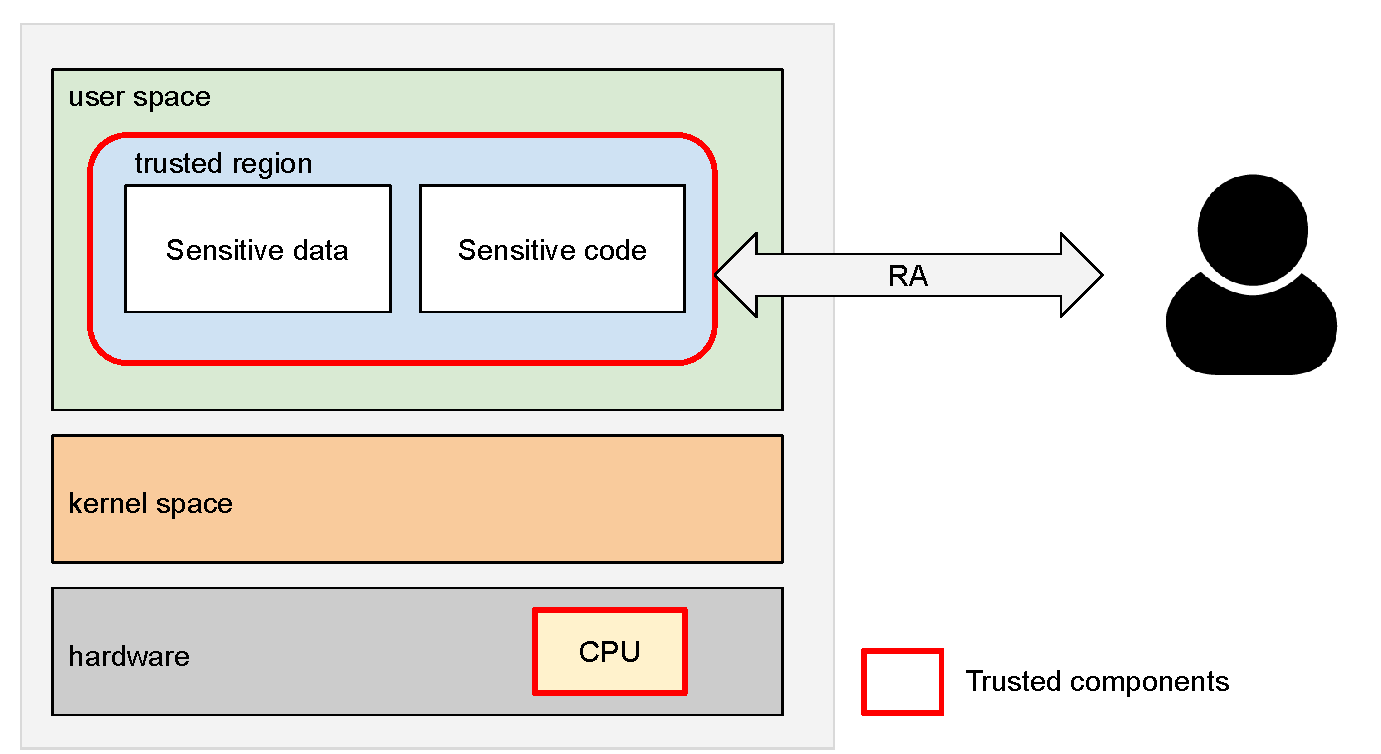
\includegraphics[width=0.7\textwidth]{fig_c1/sgx-architecture.pdf}
	\caption[SGX architecture.]{Simplified TEE architecture.}
	\label{fig:sgx-architecture}
\end{figure}

%\todo{possible solution: TEE. Give intuitive definition.}
For tackling the aforementioned challenges, a promises direction is 
represented by Trusted Execution Environments (TEE).
Intuitively, TEEs are sub-systems, whose functioning remembers virtual 
machines, that use hardware checks to isolate sensitive content against 
untrusted environments.
%\todo{Definition of TEE and usage. Properties, memory isolation, and remote 
%attestation.}
%\todo{History of TEEs, first definition, standard used, etc. During the 
%	description, stay "high level" and recall properties and differences. This 
%	should give a context.} 
Figure~\ref{fig:sgx-architecture} shows a simplified design of a TEE.
Here, the main CPU represents the primary source of trust and enables a user to 
define \emph{trusted memory regions} in the main memory 
(RAM)~\citep{Sabt2015TrustedEE}.
Historically, the first formal definition of TEE has been proposed by 
\cite{omtp}, that mainly focused on mobile platforms (\eg smartphones).
OMTP defines a list of properties that a TEE should fulfill, among them, this 
thesis will trait the \emph{memory isolation} and the \emph{remote attestation}.
The main purpose of the \emph{memory isolation} is to shield code and data such 
that even a compromised machine cannot alter its integrity and confidentiality.
In particular, the \emph{memory isolation} must prevent tampering from any 
sources at any privilege level, \eg it must avoid writing and reading 
operations from the operating system, system management mode 
code~\citep{yao2009system}, and direct memory 
access~\citep{coke1998implementing}.
The \emph{remote attestation}, instead, guarantees that a third party (\eg a 
smartphone) can verify the integrity of a remote entity (\eg a Web service).
This ensures that a client is communicating with the intended portion of code 
and machine, this latter usually represented by a CPU ID.
The combination of \emph{memory isolation} and \emph{remote attestation} leads 
to a new range of properties in the cloud environments, \ie a company 
can use the \emph{memory isolation} to protect critical piece of 
software and data from insiders or a compromised host.
%, or even other VMs sharing the same resources.
In addition, the \emph{remote attestation} allows one to establish 
end-to-end secure channels without the need of a trusted OS, thus avoiding the 
leak of cryptographic material.
In addition, the TEEs can use attestation to seal data on non-volatile storage 
(\ie encrypt and decrypt) such that nobody but the original \emph{trusted 
region} can retrieve the content. 
TEEs are peculiar technologies that differ from previous solutions, such as TPM 
ones. Specifically, TMPs require an external hardware (\ie the TPM module), 
while TEEs are embedded in the main CPU.
Moreover, TPMs do not provide memory isolation, can only store limited 
cryptographic material (\eg keys), and expose a limited number functionalities 
already wired in the module by the vendor
(\eg random number generation or cryptographic primitives).
On the contrary, TEEs contain general purpose software that might 
interact with the peripherals.
We provide a detailed TEE background in Chapter~\ref{chp:background}.
%\todo{introduce SGX at least a little bit, because I am gonna cite it later 
%on.}

%%\todo{consider to remove this part at all! why going too deep into SGX now?}
%From the first OMTP definition, many vendors proposed their own TEE technology 
%on the market.
%In 2012, Intel proposed  Trusted Execution Technology 
%(TXT) to measure the software integrity~\citep{greene2012intel}.
%In 2014, ARM introduced the TrustZone technology in new lines of CPU and 
%controllers~\citep{arm-trustzone}. 
%%TrustZone devices can bootstrap two parallel OSs: one called \emph{enriched} 
%%OS, that should handle all the normal operations; and a second one called 
%%\emph{trusted} OS, with the duty to containing critical applications.
%More recently, AMD proposed Secure Encrypted Virtualization 
%(SEV) that shields whole VMs from their host~\citep{amdsev}, likewise,
%Apple proposed a similar technology for their 
%smartphones~\citep{apple-enclave}.
Among the various technologies available on the market, one particularly 
attracted the attention of the cloud vendors: Intel Software Guard eXtensions 
(SGX).
Intel SGX was announced in 2013~\citep{rozas2013intel} and is currently 
adopted 
by many cloud providers, such as Azure~\citep{azure}, 
GCP~\citep{challita2018precise}, IBM~\citep{IBM}, and 
Alibaba~\citep{alibabasgx}.
This technology provides either a strong \emph{memory isolation} and a 
reliable 
\emph{remote attestation} that stand at the backbone of many businesses, such 
as Signal~\citep{signal}.
Due to the important growth of SGX in the recent years, and considering its 
adoption in the cloud computing market, this thesis will consider SGX as main 
TEE technology.
Nevertheless, the contributions discussed in this thesis are generic and can be 
adapted for others TEEs.
SGX calls its \emph{memory regions} as \emph{enclaves}, that reside in 
user-space, and provides a \emph{remote attestation} to validate the correct 
\emph{enclave} initialization.
We provide further details about SGX in 
Section~\ref{sec:software-guard-extension}.


%\section{Software Guard eXtensions Overview}
%
%\todo{consider to remove this part at all.}
%The architecture of Intel Software Guard eXtensions (SGX) is synthesized in 
%Figure~\ref{fig:sgx-architecture}.
%SGX assumes the whole system is compromised (\emph{untrusted}) and the 
%CPU is the only root of trust.
%In SGX machines, the kernel can uses dedicated CPU opcodes to instantiate 
%\emph{enclaves}: memory regions in user-space physically isolated from the 
%rest 
%of the system.
%The CPU monitors the correct initialization of SGX \emph{enclaves}, that are 
%thus considered \emph{trusted regions}.
%Moreover, the CPU performs extract controls that ensure \emph{enclaves} 
%\emph{memory isolation}.
%%The booting of an enclave is handled at kernel-space (\ie through a driver) 
%%in 
%%combination with extra CPU checks that ensure the correct \emph{enclave} 
%%loading.
%Once an \emph{enclave} is bootstrapped, a remote entity can perform a 
%\emph{remote attestation} (SGX RA) to verify the \emph{enclave} integrity.
%The \emph{enclaves} live only in user-space and cannot directly 
%interact with the kernel (\ie they cannot invoke \texttt{sycalls}).
%The interaction between \emph{enclaves} and OS is handed by development 
%frameworks that organize the enclave code in \emph{secure} and \emph{outside 
%functions}.
%The former are contained in the \emph{enclave} and handle critical pieces of 
%code and data, while the latter are in the \emph{untrusted region} and 
%interact 
%with the system (\eg writing files, network communication).
%We provide further details of the SGX internals in 
%Section~\ref{sec:software-guard-extension}.

\section{Problem Statement}

TEE technologies achieve a strong security level mainly thanks to
\emph{memory isolation} and \emph{remote attestation}.
At firs sight, these properties might appear as the final solution for 
cloud provider security: the former entrusts confidentiality and integrity by 
design, while the latter allows secure communication channels.
Unfortunately, as common with new technology, their adoption stimulated 
adversaries to develop new intrusion techniques.
Moreover, these properties suffer from technical limitations that require 
researchers to overcome new challenges.
For instance, TEEs often provide a limited amount of isolated memory, thus 
arising scalability issues.
Or else, an adversary may take advantage of the memory isolation to develop new 
intrusion techniques.
If this happens, detecting threats hidden in trusted regions becomes crucial.
In addition, the current integrity mechanisms are limited to static properties 
(\ie if a piece of code is intact) while overlooking runtime attacks (\eg 
code-reuse ones).
Only few recent solutions investigated such threats, but their design is 
limited to embedded systems.
This section digs into the main issues that afflict \emph{memory 
isolation} and \emph{remote attestation}.

\subsection{Memory Isolation}

An ideal \emph{memory isolation} is enforced at hardware level with new CPU 
opcodes and extra checks at microcode level, thus having an OS independent 
design.
If this property effectively protects against compromised hosts, the isolation 
also introduces new challenges.
For instance, handling the interaction between the trusted region and 
the external word (\eg to write a file) assumes a new programming patter.
From the security perspective, un-observable portions of memory may help an 
adversary to hide its presence in the machine.
In the following, we elaborate these limitations of \emph{memory isolation}.

\vspace{0.5cm}
\noindent \textbf{Memory limit and scalability problems.}
In TEE technologies, and in particular SGX \citep{costan2016intel}, the 
software within a \emph{trusted region} cannot directly interact with the 
hosting OS, moreover, the \emph{trusted region} often has a limited 
size~\citep{baumann2015shielding}.
Previous works studied solutions that move part of the OS functionality inside 
a \emph{trusted 
region}~\citep{baumann2015shielding,arnautov2016scone,tsai2017graphene},
but they introduce further complexity for employing a secure interaction with 
the rest of the world (\eg networking, file system).
Other authors suggested protecting only critical portions of the 
code \citep{schuster2015vc3,lind2017glamdring}.
However, these approaches do not address critical limitations such as the 
interaction with the underlying OS, or the limited amount of memory.
Limited memory makes it unsustainable to deploy all processes in dedicated 
trusted containers.
For instance, machines featured with SGX provide only a few hundred megabytes 
that must be shared among all the running \emph{enclaves}.
If we consider processes such as Skype or Firefox, which require around 
$100$MB each, we need multiple \emph{enclaves} for each process to protect.
Therefore, this approach does not scale for multiple parallel processes.
The introduction of SGX $2.0$ allows modifying the size of a single trusted 
container but it does not modify the maximum memory available for trusted 
containers.
Therefore, we require alternative solutions to overcome the scalability issues 
affecting \emph{trusted regions}.

\vspace{0.5cm}
\noindent \textbf{TEEs as a nest for new threats.}
%
%The SGX design, coupled with a full encryption of an enclave's content, 
%provides advanced protection mechanisms and a trusted communication channel 
%between the enclave and the host process (\ie the main application the enclave 
%belongs to).
%The success of SGX stems from its strict threat model, that considers the OS
%malicious: one can thus tamper with applications, modify their
%behavior, exfiltrate sensitive information, and so on~\citep{iagoattack}.
%In this context, SGX disallows kernel- and user-space code to
%manipulate enclave memory pages, thus guaranteeing integrity and
%confidentiality in the presence of any Iago attacker.
%
The strong isolation introduced by TEE technologies stimulated researchers and 
practitioners to develop new attacks 
vectors~\citep{foreshadow,Murdock2019plundervolt,203183,lee2017hacking}.
Among them, an interesting research line is to exploit memory-corruption 
errors inside the \emph{trusted regions} and run one-shot code-reuse attacks to 
steal enclave secrets (\eg cryptographic keys)~\citep{geometry2007}.
Recently, we observed many solutions that identify such flaws in \emph{trusted 
regions}~\citep{teerex,tale-two-worlds} and specifically new code-reuse 
techniques tailored for SGX~\citep{lee2017hacking,biondo2018guard}.
%First, \cite{lee2017hacking} discussed Dark-ROP that combines a colluded OS 
%and 
%oracles to identify gadgets for return-oriented programming 
%(ROP)~\citep{geometry2007}.
%The main limitation of this attack is the need of crashing the victim
%enclave many times in order to craft the actual payload.
%%An advanced technique was proposed by \cite{biondo2018guard} with Guard's 
%%Dilemma that does not require the assistance of the OS 
%%to perform the attack.
%To cope with this issue, \cite{biondo2018guard} proposed Guard's 
%Dilemma that uses particular gadgets already present in the Intel Software 
%Development Kit (SDK) to build the payload without any enclave crashes.
%Moreover, Dilemma requires only an unprivileged attacker to carry out a 
%single one-shot attack and steal secrets from an enclave.
In this scenario, an adversary may craft an attack that bypass 
existing memory forensic techniques and hide its presence in a legitimate 
\emph{trusted region}.
%
%to identify the 
%intrusions~\citep{stancill2013check,polychronakis2011rop,kittel2015counteracting,Graziano:2016:RFA:2897845.2897894}.
For instance, in case of external intrusion into a remote server running SGX 
enclaves, the adversary could infect an \emph{enclave}, use it to 
perpetrate actions against the system, and hide her presence behind the 
\emph{memory isolation}.
We thus need to understand which conditions lead to these new threats and to 
what extent they might spread in real scenarios.
% is also interested in reducing the amount of traces 
%left; otherwise, analysts may detect the intrusion and act consequently.
%This is even more critical in case the enclave secret changes and the 
%adversary has to repeat the attack many times.

\vspace{0.5cm}
\noindent \textbf{Incident investigation issues.}
The strong isolation provided by TEE technologies is a double-edged
sword --- protecting legitimate code from untrusted environments,
but also preventing security tools from inspecting the memory and performing
forensic investigations. 
As a result, both researchers and malware developers have also investigated how 
to exploit TEEs for malicious purposes 
\citep{thoughs-on-intel1,thoughs-on-intel2,sgxrop,snakegx,sgxsidechannel}.
Even though code running in a \emph{trusted region} cannot be retrieved and 
analyzed, other artifacts may be present in unprotected memory, thus allowing 
an investigator to infer certain properties of what is running inside the 
protected space.
In fact, a \emph{trusted region} cannot be completely self-contained, as it 
always needs some external support code to interact with the rest of the 
environment.
However, to the best of our knowledge, no study has been performed to date on 
the consequences of TEEs on memory forensics.

\subsection{Remote Attestation}

In standard Remote Attestation (RA) schemes, usually defined as static, the 
\emph{Prover} verifies the integrity of specific hardware and 
software properties -- the \emph{Prover} has loaded the correct software.
%On the market, there are already several available products implementing 
%static RA, such as Software Guard Extensions (SGX)~\citep{costan2016intel} or 
%Trusted Platform Module (TPM)~\citep{tomlinson2017introduction}.
Intuitively, these do not protect against runtime attacks (\eg the 
control-flow ones) that aim to modify the program runtime behaviour. 
Therefore, to identify \emph{Prover} runtime modifications, researchers 
proposed runtime RA.
In the literature, a common runtime RA assumption is to rely on a \emph{trusted 
region} to track events from an application, this latter might also reside in 
the \emph{untrusted region}, while the \emph{trusted region} is considered as 
out of the attacker range.
Unfortunately, the current runtime RAs show some limitations.
%Among the different solutions belonging to this category, 
%there are also the control-flow attestation approaches, which
%encode the information about the executed control-flow of a 
%process~\citep{abera2016c,aberadiat}.

\vspace{0.5cm}
\noindent \textbf{Runtime Remote Attestation do not Scale over Complex System.}
The main runtime RAs from the literature mainly focus on embedded 
devices~\citep{abera2016c,zeitouni2017atrium,aberadiat,dessouky2017fat,Dessouky:2018:LLH:3240765.3240821}:
most of them encode the complete execution path of a \emph{Prover} in a single 
hash~\citep{abera2016c,zeitouni2017atrium,dessouky2017fat}; 
some relies on a policy-based verification schema~\citep{aberadiat}; and0
other ones adopt symbolic execution to verify the control-flow information 
sent by the \emph{Prover}~\citep{Dessouky:2018:LLH:3240765.3240821}.

Even though the previous solutions result suitable for embedded devices, none 
of them can be applied to a complex system due to the following reasons: 
\begin{enumerate*}[label=(\roman*)]
	\item representing all the valid execution paths through hash values is 
	unfeasible (\eg the number of execution paths tends to grow exponentially 
	with the size of the program),
	\item the policy-based approaches might not cover all the possible attacks,
	\item symbolic execution slows down the verification phase.
\end{enumerate*}
Therefore, we need a new model that tackles these challenges and can represent 
complex software in limited space, thus being able to be adopted in cloud 
infrastructures. 
%We describe our study in Chapter~\ref{chp:runtime-protection-untrusted}.

\vspace{0.5cm}
\noindent \textbf{Runtime Remote Attestation do not Work on TEEs.}
Runtime RAs assume a TEE to trace the application execution.
Therefore, we cannot directly deploy a runtime RA in a TEE because the 
\emph{memory isolation} would block any tracing of the \emph{trusted regions}.
%TEE guarantees a \emph{trusted region} is properly loaded in memory, while 
%static RA allows a remote entity to verify the correct enclave initialization.
As such, the TEE alone has no mechanisms to guarantee the correct runtime 
execution of a \emph{trusted region}, which remain vulnerable against
attacks aimed at causing deviations from enclaves' expected legitimate
behaviors~\citep{tale-two-worlds,251582,biondo2018guard,lee2017hacking,snakegx}.
The \emph{memory isolation} exacerbates runtime attacks that target 
software loaded in \emph{trusted regions}, since there is no mechanism to 
monitor their executions and set legitimate and anomalous ones apart.
Although one can adopt mechanisms tailored at counteracting 
specific threats, research has shown such solutions are brittle and cover a 
limited threat model, mostly focusing on code-reuse attacks, while neglecting 
vectors that induce deviation from normal
behaviors~\citep{tale-two-worlds,251582,biondo2018guard,lee2017hacking}.
Moreover, current runtime remote attestations focus on
stateless properties, \ie they only model independent executions.  On
the contrary, TEEs are stateful objects modeled as finite states
machines (FSM), as described by \cite{costan2016intel}.
Finally requiring more complex representations.
Considering all these limitations, we need a runtime RA that can be employed in 
\emph{trusted regions}.

\section{Thesis Contributions}

\begin{figure}[t]
	\centering
	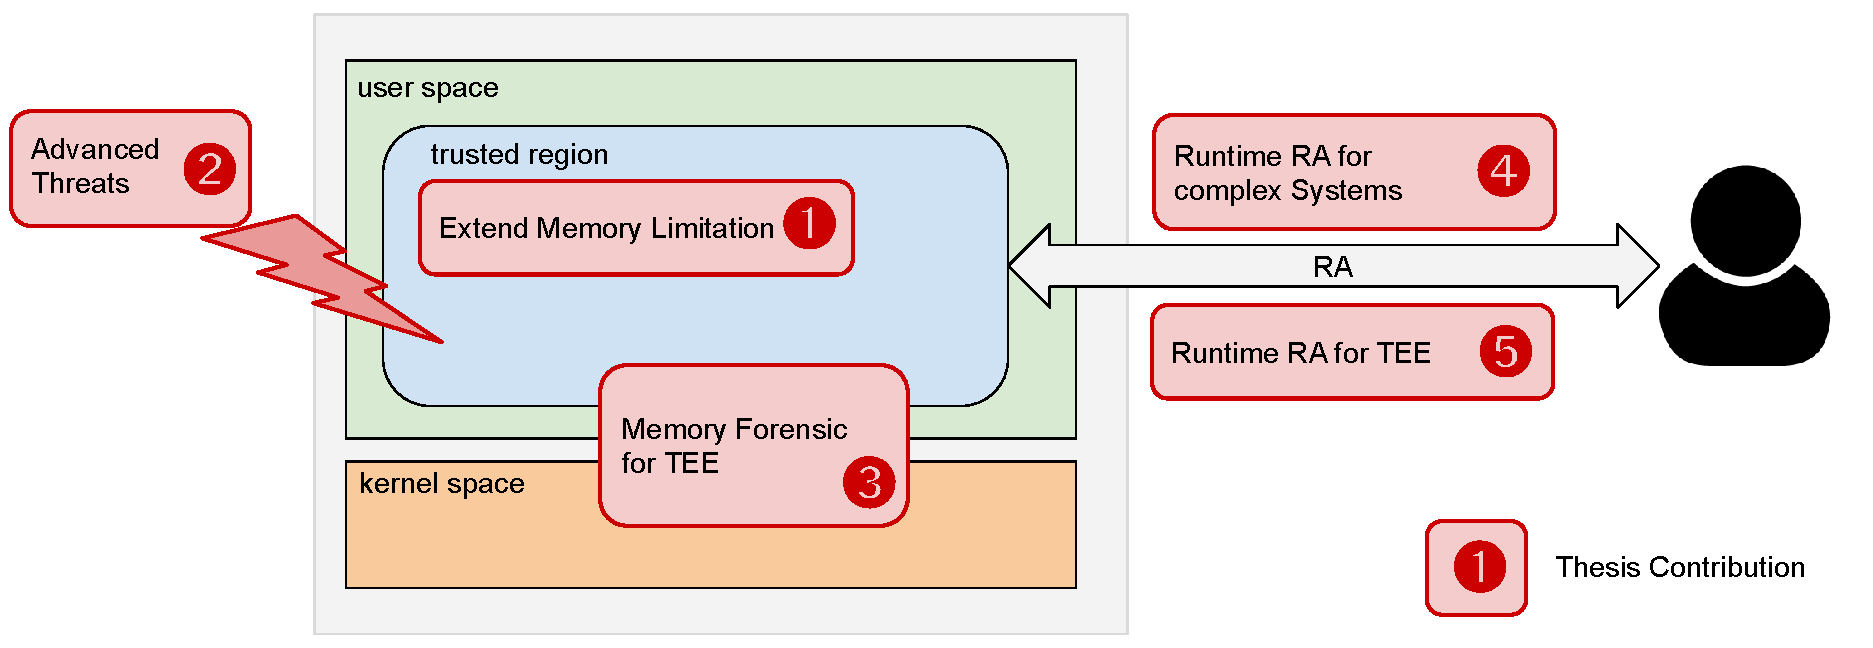
\includegraphics[width=\textwidth]{fig_c1/contribution.pdf}
	\caption[Thesis contribution.]{Thesis contribution.}
	\label{fig:contribution}
\end{figure}

Regardless the security guarantees achieved by TEEs, their design still 
suffers from important limitations.
The object of this thesis is
%% THESIS OBJECTIVE - FIRST VERSION
In this thesis, we argue we can improve the TEE security level
through a shrewd software design without the need of changing the hardware 
specification.
Specifically, we identify five main challenges to investigate and for each of 
them we propose specific contributions.
%The thesis will describe five contributions in total that will 
%address four aspect of SGX. 
The whole thesis contribution is depicted in 
Figure~\ref{fig:contribution}, that we summarize here and further elaborate in 
dedicated chapters.

\begin{itemize}
	\item[\circledrA{1}] \textbf{Extend Memory Isolation.}
	In TEE machines, usually the space for trusted memory regions is bounded 
	to few mega bytes. 
	This affects the amount of critical content that can be protected 	
	contemporaneously.
	In Chapter~\ref{chp:static-protection}, we study a new software design that 
	stretches the TEE \emph{memory isolation} over vaster memory areas while 
	keeping a limited overhead.
%	This is depicted by the symbol \circledr[1] in 
%	Figure~\ref{fig:contribution}.
	
	\item[\circledrA{2}] \textbf{Advanced Threats Led by Memory Isolation.} The 
	\emph{memory isolation} avoids an external observer to understand the 
	internal behavior of a TEE. Therefore, this isolated space could 
	be used as a nest for a new category of malware.
	In Chapter~\ref{chp:advanced-threats}, we study to which extent an 
	adversary can exploit the TEE isolation to introduce new treats in a system.
%	This is depicted by the symbol \circledr[2] in 	
%	Figure~\ref{fig:contribution}.

	\item[\circledrA{3}]
	\textbf{Incident Response Limitations.} The introduction of 
	non-observable memory regions affects the incidents response in 
	case of intrusion.
	In Chapter~\ref{chp:forensic}, we study the limitation of current 
	investigation techniques in the context of TEE machines and propose new 
	memory-forensic methodologies to investigate the intrusions in these 
	systems.
	
	\item[\circledrA{4}]
	\textbf{Scalable Runtime Remote Attestation for Complex Systems.}
	Current Runtime RA schemes are meant for relatively simple pieces of 
	software in embedded systems.
	In cloud scenarios, where a VM could load programs of any complexity, the 
	current solutions suffer from scalability issues.
	In Chapter~\ref{chp:runtime-protection-untrusted}, we study a new scalable 
	runtime RA schemes that can be deployed over 
	complex systems typical of cloud computing.
%	This is depicted by the symbol \circledr[3] in 
%	Figure~\ref{fig:contribution}.
	
	\item[\circledrA{5}]
	\textbf{Runtime Remote Attestation for TEE.} 
	The standard RA can only guarantee that a TEE has been 
	loaded properly, but it does not model runtime properties such as the 
	execution-flow or the internal state.
	Unfortunately, current runtime RA cannot be deployed inside the TEE space
	for mainly two reasons: (i) the memory isolation disallows tracing TEE
	runtime information, and (ii) TEEs are stateful objects that cannot be 
	modeled with current runtime RA schemes.
	In Chapter~\ref{chp:runtime-protection-trusted}, we propose a new RA schema 
	that is suitable for TEEs.
%	This is depicted by the symbol \circledr[4] in 
%	Figure~\ref{fig:contribution}.
	
%	This is depicted by the symbol \circledr[5] in 	
%	Figure~\ref{fig:contribution}.
\end{itemize}

\section{Outline}
\label{sec:outline}

Here, the thesis' outline.

\begin{itemize}[label={}]
	\item \textbf{Chapter~\ref{chp:background}:} We provide background 
	knowledge about TEEs and the main attack vectors discussed in the thesis.
	\item \textbf{Chapter~\ref{chp:static-protection}:} We propose our solution 
	to overcome memory-constraints in TEEs.
	\item \textbf{Chapter~\ref{chp:advanced-threats}:} We describe our 
	technique to infect legitimate \emph{trusted regions}.
	\item \textbf{Chapter~\ref{chp:forensic}:} We investigate the capabilities 
	of 	memory-forensic techniques in TEE machines.
	\item \textbf{Chapter~\ref{chp:runtime-protection-untrusted}:} We 
	illustrate our new model to improve scalability in runtime RAs.
	\item \textbf{Chapter~\ref{chp:runtime-protection-trusted}:} We detail our 
	new model to implement a runtime RA inside a TEE.
	\item \textbf{Chapter~\ref{chp:related-works}:} We compare our results 
	with the literature.
	\item \textbf{Chapter~\ref{chp:conclusion}:} We discuss the contribution 
	introduced in the thesis and conclude.
\end{itemize}

%\begin{figure}[t]
%	\centering
%	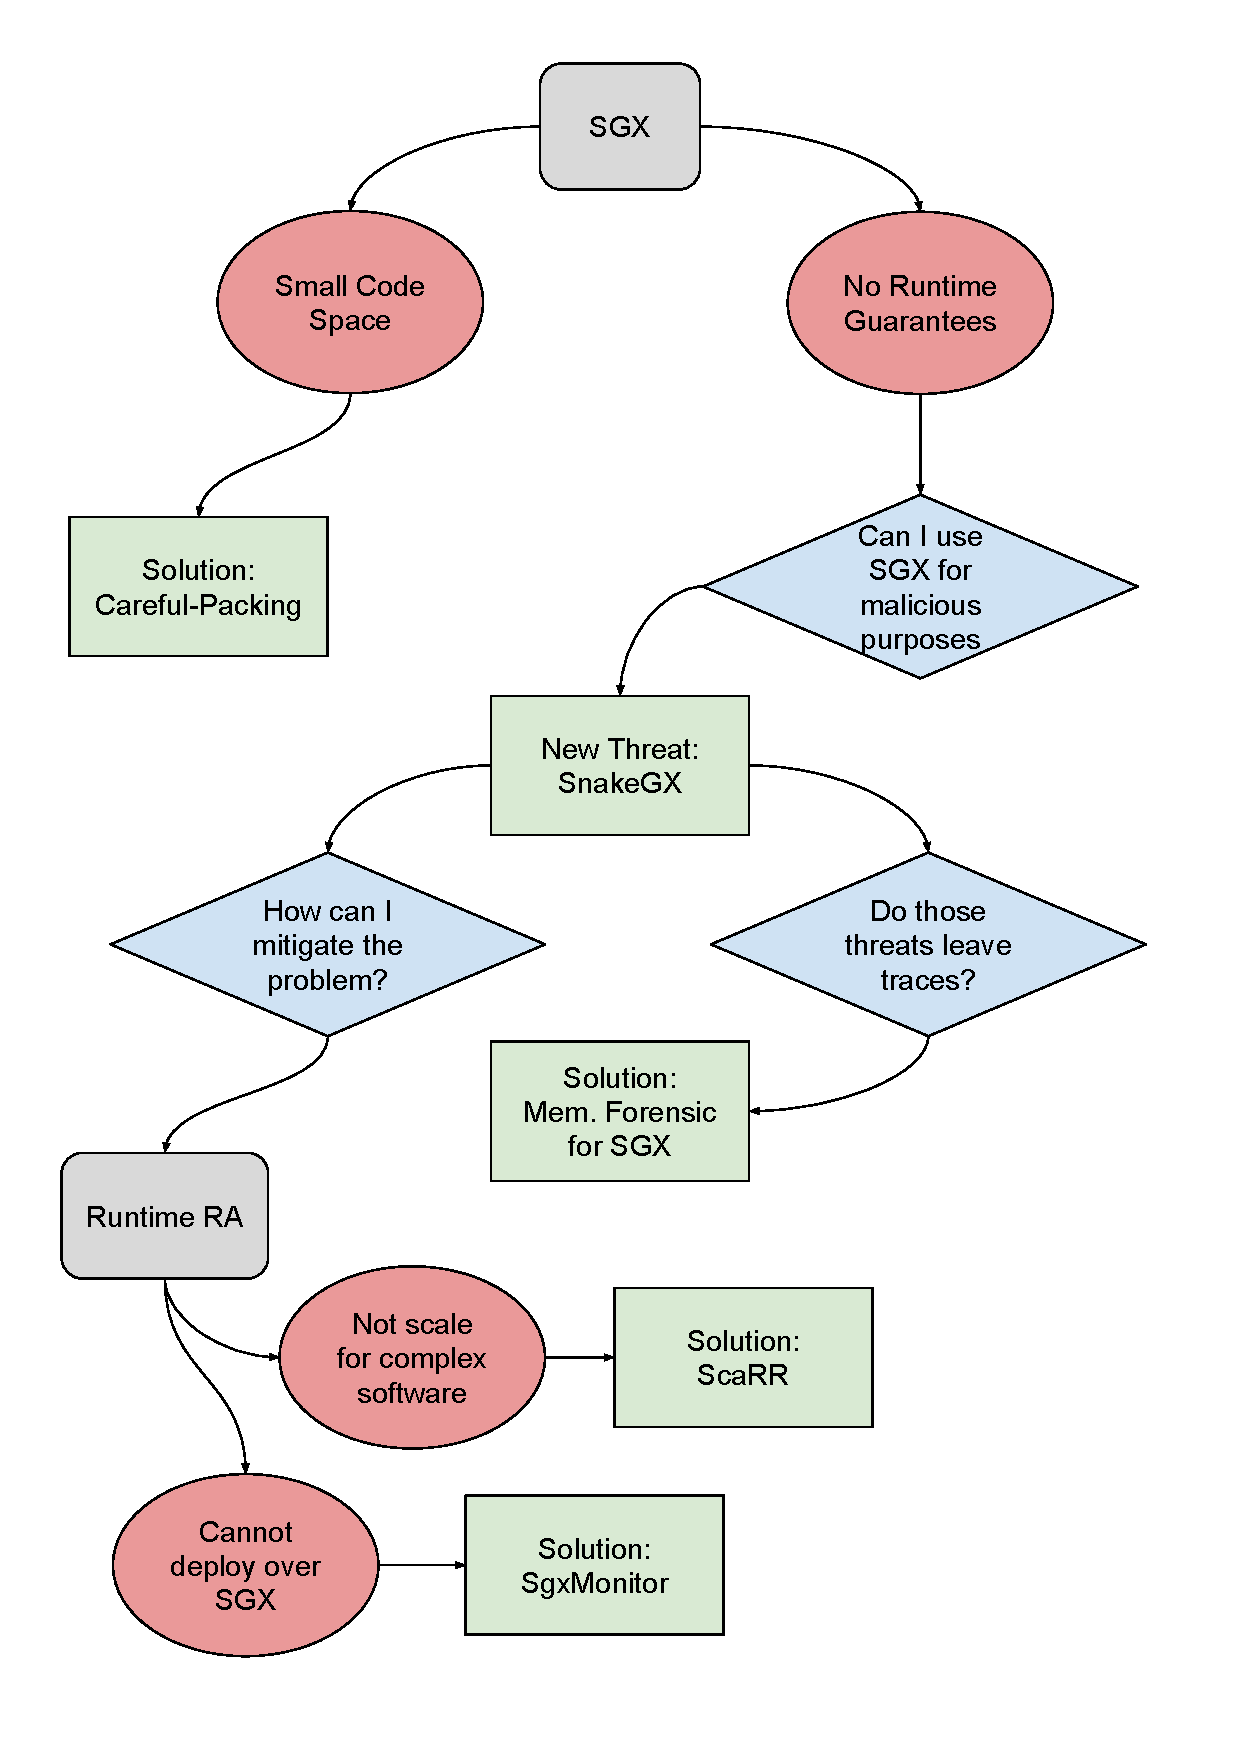
\includegraphics[width=\textwidth]{fig_c1/mind-map.pdf}
%	\caption[Mind-map.]{Mind-map (TO REMOVE LATER).}
%	\label{fig:mind-map}
%\end{figure}

%
%\subsection{Extend Enclaves Memory Limitations}
%\label{ssec:contribution1}
%
%The \emph{memory isolation} of TEE modules is a strong protection against 
%tampering attacks, which are commonly model as Man-At-The-End adversary (MATE).
%In this scenario, the adversary may edit the binary code to alter the process 
%logic~\citep{AKHUNZADA201544}, while the defender must guarantee that an 
%adversary cannot change the software logic to some extent. 
%TEE technologies, and in particular SGX, provide \emph{enclaves} 
%that shield the software, thus avoiding MATE by design~\citep{costan2016intel}.
%However, TEEs often have practical limitations, \eg software within an 
%\emph{enclave} cannot directly interact with the hosting OS; and the enclave 
%often has size limitations~\citep{baumann2015shielding}.
%Previous works studied solutions that move part of the OS functionality inside 
%a \emph{trusted 
%region}~\citep{baumann2015shielding,arnautov2016scone,tsai2017graphene},
%but they introduce further complexity for employing a secure interaction with 
%the rest of the world (\eg networking, file system).
%Other authors suggested protecting only portions of the 
%code~\cite{schuster2015vc3,lind2017glamdring}.
%However, these approaches do not address critical limitations such as the 
%interaction with the underlying OS, or the limited amount of memory.
%Limited memory makes it unsustainable to deploy all processes in dedicated 
%trusted containers.
%For instance, machines featured with SGX provide only a few hundred megabytes 
%that must be shared among all the running \emph{enclaves}.
%If we consider processes such as Skype or Firefox, which require around 
%$100$MB each, we need multiple \emph{enclaves} for each process to protect.
%Therefore, this approach does not scale for multiple parallel processes.
%The introduction of SGX $2.0$ allows modifying the size of a single trusted 
%container but it does not modify the maximum memory available for trusted 
%containers.
%
%As an alternative approach, researchers proposed anti-tampering techniques, 
%that allow a software to inspect itself and check whether its code has been 
%modified.
%We refer to those techniques as \emph{self-checking}, which literally read the 
%binary code of the protected software by using special functions called 
%\emph{checkers}.
%The checkers compute a digital fingerprint of the software bytecode and verify 
%whether that fingerprint matches a pre-computed 
%value~\citep{nagra2009surreptitious}. 
%However, purely software-based anti-tampering techniques are not 
%completely secure, since the defending mechanisms reside in an 
%\emph{untrusted memory region} and a determined attacker can identify and 
%disarm such defenses.
%It is possible to harden anti-tampering techniques by using a combination of 
%additional 
%approaches that raise the bar for the attackers but that do not fundamentally 
%address the 
%problem~~\citep{horne2001dynamic,banescu2017tutorial,chen2016advanced,chang2001protecting,viticchie2016reactive}
%
%Considering all the aforementioned problems, we propose to combine the 
%anti-tampering techniques and the SGX isolation to extend code protection over 
%\emph{untrusted region}.
%Finally overcoming the intrinsic limitations of SGX.
%We detail our contribution in Chapter~\ref{chp:static-protection}.
%
%\subsection{Investigating New Threats Led by Memory Isolation}
%\label{ssec:contribution2}
%
%The SGX design, coupled with a full encryption of an enclave's content, 
%provides
%advanced protection mechanisms and a trusted communication channel between the
%enclave and the host process (\ie the main application the enclave belongs to).
%The success of SGX stems from its strict threat model, that considers the OS
%malicious: one can thus tamper with applications, modify their
%behavior, exfiltrate sensitive information, and so on~\citep{iagoattack}.
%In this context, SGX disallows kernel- and user-space code to
%manipulate enclave memory pages, thus guaranteeing integrity and
%confidentiality in the presence of any Iago attacker.
%
%The strong isolation introduced by SGX stimulated researchers and 
%practitioners 
%to develop new attacks 
%vectors~\citep{foreshadow,Murdock2019plundervolt,203183,lee2017hacking}.
%Among them, an interesting research line is to exploit memory-corruption 
%errors inside the enclave code and run one-shot code-reuse attacks to steal 
%enclave secrets (\eg cryptographic keys)~\citep{geometry2007}.
%Recently, we observed many solutions that identify such flaws in 
%enclaves~\citep{teerex,tale-two-worlds} and new code-reuse techniques 
%tailored for SGX~\citep{lee2017hacking,biondo2018guard}.
%First, \cite{lee2017hacking} discussed Dark-ROP that combines a colluded OS 
%and 
%oracles to identify gadgets for return-oriented programming 
%(ROP)~\citep{geometry2007}.
%The main limitation of this attack is the need of crashing the victim
%enclave many times in order to craft the actual payload.
%%An advanced technique was proposed by \cite{biondo2018guard} with Guard's 
%%Dilemma that does not require the assistance of the OS 
%%to perform the attack.
%To cope with this issue, \cite{biondo2018guard} proposed Guard's 
%Dilemma that uses particular gadgets already present in the Intel Software 
%Development Kit (SDK) to build the payload without any enclave crashes.
%Moreover, Dilemma requires only an unprivileged attacker to carry out a 
%single one-shot attack and steal secrets from an enclave.
%
%
%In this scenario, however, the previous authors did not consider an OS that 
%may 
%employ existing memory forensic techniques to identify the 
%intrusions~\citep{stancill2013check,polychronakis2011rop,kittel2015counteracting,Graziano:2016:RFA:2897845.2897894}.
%For instance, in case of external intrusion into a remote server running SGX 
%enclaves, the adversary is also interested in reducing the amount of traces 
%left; otherwise, analysts may detect the intrusion and act consequently.
%This is even more critical in case the enclave secret changes and the 
%adversary 
%has to repeat the attack many times.
%
%Considering all these challenges and the current state-of-the-art, we 
%investigate if TEEs (and SGX in particular) can help adversaries carry more 
%advanced threats by exploiting the TEE \emph{memory isolation}.
%We detail our study in Chapter~\ref{chp:advanced-threats}.
%
%\subsection{Remote Attestation for Complex Systems}
%\label{ssec:contribution3a}
%
%\subsection{Remote Attestation for SGX}
%\label{ssec:contribution3b}
%
%In standard Remote Attestation (RA) schemes, usually defined as static, the 
%\emph{Prover} verification involves the integrity of specific hardware and 
%software properties (\eg the \emph{Prover} has loaded the correct software).
%On the market, there are already several available products implementing 
%static RA, such as Software Guard Extensions (SGX)~\citep{costan2016intel} or 
%Trusted Platform Module (TPM)~\citep{tomlinson2017introduction}.
%However, these do not provide a defence against runtime attacks (\eg the 
%control-flow ones) that aim to modify the program runtime behaviour. 
%Therefore, to identify \emph{Prover} runtime modifications, researchers 
%proposed runtime RA. Among the different solutions belonging to this category, 
%there are also the control-flow attestation approaches, which
%encode the information about the executed control-flow of a 
%process~\citep{abera2016c,aberadiat}.
%
%Studying the runtime RAs available in the literature, we identify two main 
%limitations worthy of attention. 
%First, we observed that current RAs are not suitable for complex systems, such 
%as software running in cloud infrastructures.
%Second, the current solutions cannot be employed in TEE technologies, such as 
%SGX.
%In the following, we explore these two limitations.
%
%\paragraph{Runtime RA for Complex Systems.} 
%
%In comparison to static RA, the runtime one is relatively new, and today there 
%are no reliable products available on the market since researchers have mainly 
%investigated runtime RA for embedded 
%devices~\citep{abera2016c,zeitouni2017atrium,aberadiat,dessouky2017fat,Dessouky:2018:LLH:3240765.3240821}:
%most of them encode the complete execution path of a \emph{Prover} in a single 
%hash~\citep{abera2016c,zeitouni2017atrium,dessouky2017fat}; 
%some~\citep{aberadiat} compress it in a simpler representation and rely on a 
%policy-based verification schema; 
%other ones~\citep{Dessouky:2018:LLH:3240765.3240821} adopt symbolic execution 
%to verify the control-flow information continuously sent by the \emph{Prover}.
%
%Even though the previous solutions result suitable for embedded devices, none 
%of them can be applied to a complex system due to the following reasons: 
%\begin{enumerate*}[label=(\roman*)]
%	\item representing all the valid execution paths through hash values is 
%	unfeasible (\eg the number of execution paths tends to grow exponentially 
%	with the size of the program),
%	\item the policy-based approaches might not cover all the possible attacks,
%	\item symbolic execution slows down the verification phase.
%\end{enumerate*}
%Therefore, we study a new model that tackle these challenges and can represent 
%complex software in limited space, thus can be adopted in cloud 
%infrastructures. 
%We describe our study in Chapter~\ref{chp:runtime-protection-untrusted}.
%
%
%\paragraph{Runtime RA for SGX.}
%
%SGX guarantees a \emph{trusted region} is properly loaded in memory, while 
%static RA allows a remote entity to verify the correct enclave initialization.
%As such, the SGX alone has no mechanisms to guarantee the correct runtime 
%execution of enclaves, which remain vulnerable against
%attacks aimed at causing deviations from enclaves' expected legitimate
%behaviors~\citep{tale-two-worlds,251582,biondo2018guard,lee2017hacking,snakegx}.
%
%The SGX \emph{memory isolation} exacerbates runtime attacks that target 
%software loaded in enclaves, since there is no mechanism to 
%monitor their executions and set legitimate and anomalous ones apart.
%Although one can equip the enclaves with mechanisms tailored at counteracting 
%specific threats, research has shown such solutions are brittle and cover a 
%limited threat model, mostly focusing on code-reuse attacks, while neglecting 
%vectors that induce deviation from normal
%behaviors~\citep{tale-two-worlds,251582,biondo2018guard,lee2017hacking}.
%Moreover, current runtime remote attestations focus on
%stateless properties, \ie they only model independent executions.  On
%the contrary, TEEs are stateful objects modeled as finite states
%machines (FSM), as described by \cite{costan2016intel}.
%Therefore, they require more complex representations.
%
%After observing all these limitations, we study a runtime RA that can be
%employed in SGX enclaves. We describe our study in 
%Chapter~\ref{chp:runtime-protection-trusted}.
%
%\subsection{Incident Response Limitations}
%\label{ssec:contribution4}
%
%Then addressed in Chapter~\ref{chp:forensic}.

